% Digital Logic Report Template
% Created: 2020-01-10, John Miller

%==========================================================
%=========== Document Setup  ==============================

% Formatting defined by class file
\documentclass[11pt]{article}

% ---- Document formatting ----
\usepackage[margin=1in]{geometry}	% Narrower margins
\usepackage{booktabs}				% Nice formatting of tables
\usepackage{graphicx}				% Ability to include graphics

%\setlength\parindent{0pt}	% Do not indent first line of paragraphs 
\usepackage[parfill]{parskip}		% Line space b/w paragraphs
%	parfill option prevents last line of pgrph from being fully justified

% Parskip package adds too much space around titles, fix with this
\RequirePackage{titlesec}
\titlespacing\section{0pt}{8pt plus 4pt minus 2pt}{3pt plus 2pt minus 2pt}
\titlespacing\subsection{0pt}{4pt plus 4pt minus 2pt}{-2pt plus 2pt minus 2pt}
\titlespacing\subsubsection{0pt}{2pt plus 4pt minus 2pt}{-6pt plus 2pt minus 2pt}

% ---- Hyperlinks ----
\usepackage[colorlinks=true,urlcolor=blue]{hyperref}	% For URL's. Automatically links internal references.

% ---- Code listings ----
\usepackage{listings} 					% Nice code layout and inclusion
\usepackage[usenames,dvipsnames]{xcolor}	% Colors (needs to be defined before using colors)

% Define custom colors for listings
\definecolor{listinggray}{gray}{0.98}		% Listings background color
\definecolor{rulegray}{gray}{0.7}			% Listings rule/frame color

% Style for Verilog
\lstdefinestyle{Verilog}{
	language=Verilog,					% Verilog
	backgroundcolor=\color{listinggray},	% light gray background
	rulecolor=\color{blue}, 			% blue frame lines
	frame=tb,							% lines above & below
	linewidth=\columnwidth, 			% set line width
	basicstyle=\small\ttfamily,	% basic font style that is used for the code	
	breaklines=true, 					% allow breaking across columns/pages
	tabsize=3,							% set tab size
	commentstyle=\color{gray},	% comments in italic 
	stringstyle=\upshape,				% strings are printed in normal font
	showspaces=false,					% don't underscore spaces
}

% How to use: \Verilog[listing_options]{file}
\newcommand{\Verilog}[2][]{%
	\lstinputlisting[style=Verilog,#1]{#2}
}




%======================================================
%=========== Body  ====================================
\begin{document}

\title{ELC 2137 Lab \06: MUX and 7-segment Decoder}
\author{Spencer Stinson}

\maketitle


\section*{Summary}

In this experiment, we learned the design and code for a multiplexer, decoder, and how to put these both into one more complex design. We also learned to use this design with a physical board. We used new syntax that we had previously not had use for, for example; always@*, for, and case. To apply this design to the FPGA, we also had to learn how to use constraints and how to run synthesis and implementations, as well as to generate a bitstream.


\section*{Q\&A}
\begin {itemize}
\item List the errors found during simulation. What does this tell you about why we run simulations?\\
One of my main errors was in naming. I consistently had an input or output name slightly different than it was meant to be. This caused me many problems and also caused my Basys board not to run correctly originally. There were also errors with the connections of some of the wires, which I only found by examining the test benches. 
\item How many wires are connected to the 7-segment display? If the segments were not all connected together, how many wires would there have to be? Why do we prefer the current method vs. seperating all of the segments?\\
There are 5 wires connected to the 7-segment display. If the segments were not all connected together, there would be 29 wires. We prefer the current method because it is much more efficient and it allows us to do all of this in less steps, as we are doing the same thing to each bit, so doing it all individually would be repetitive and cause more probability for error. 
\end{itemize}



\section*{Code}


\Verilog[caption= mutiplexer code]{C:/Users/spencer_stinson1/Documents/GitHub/Lab06A/Lab06_/Lab06_.srcs/sources_1/new/mux4_2b.sv}
\Verilog[caption= multiplexer test bench code]{C:/Users/spencer_stinson1/Documents/GitHub/Lab06A/Lab06_/Lab06_.srcs/sim_1/new/mux4_2b_testbench.sv}
\Verilog[caption= 7 segment decoder code]{C:/Users/spencer_stinson1/Documents/GitHub/Lab06A/Lab06_/Lab06_.srcs/sources_1/new/sseg_decoder.sv}
\Verilog[caption= 7 segment decoder testbench code]{C:/Users/spencer_stinson1/Documents/GitHub/Lab06A/Lab06_/Lab06_.srcs/sim_1/new/sseg_decoder_testbench.sv}
\Verilog[caption= 7 segment code]{C:/Users/spencer_stinson1/Documents/GitHub/Lab06A/Lab06_/Lab06_.srcs/sources_1/new/sseg1_.sv}
\Verilog[caption= 7 segment wrapper code]{C:/Users/spencer_stinson1/Documents/GitHub/Lab06A/Lab06_/Lab06_.srcs/sources_1/new/sseg1_wrapper.sv}
\Verilog[caption= 7 segment testbench code]{C:/Users/spencer_stinson1/Documents/GitHub/Lab06A/Lab06_/Lab06_.srcs/sim_2/new/sseg_1_testbench.sv}

\section*{Results}

\begin{figure}
	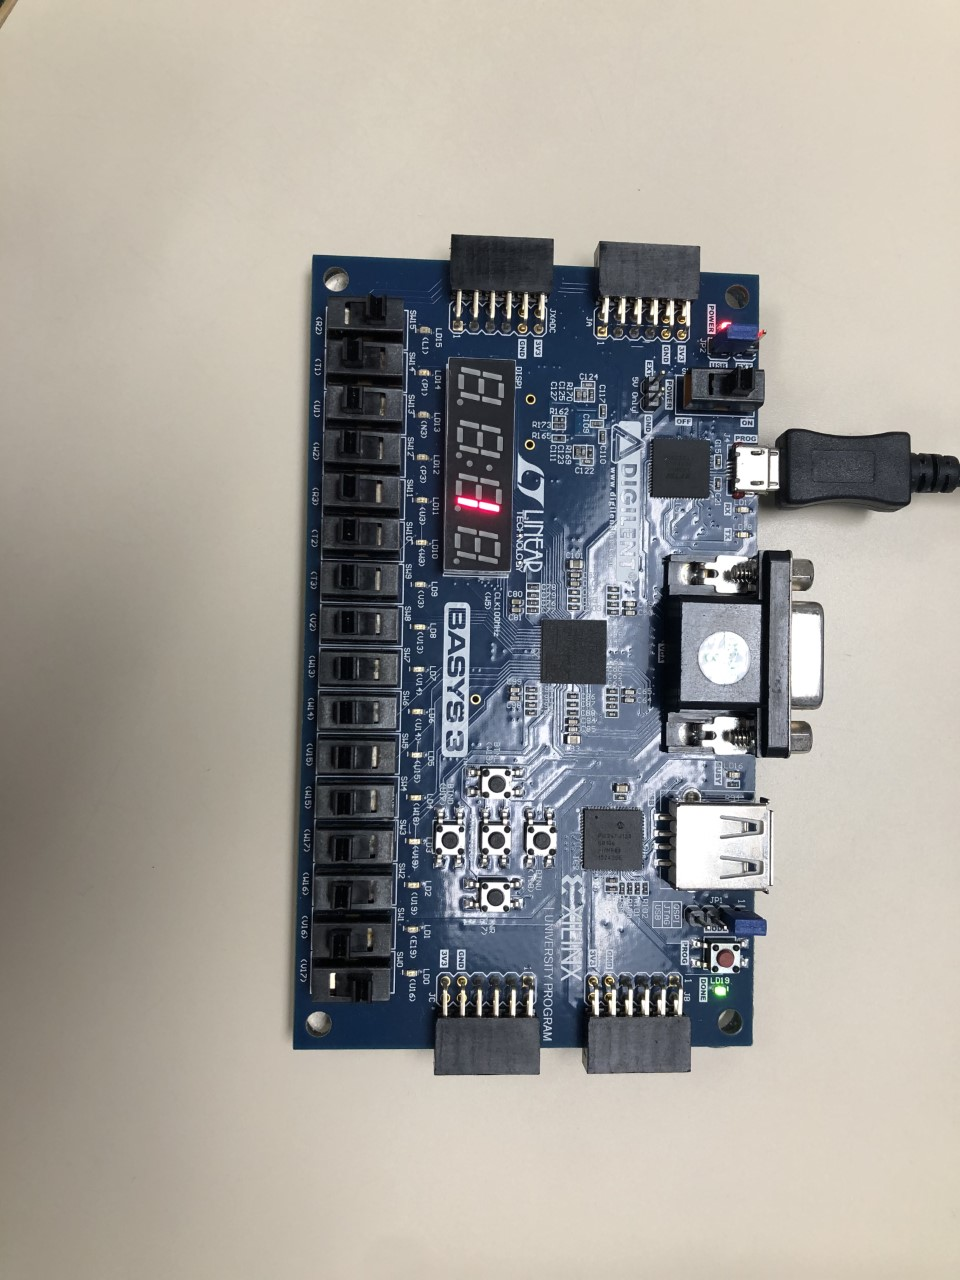
\includegraphics[width= \textwidth]{basys.png}
	\caption{Basys board running 7 segment on second display }\label{fig:Basys}
\end{figure}
\begin{figure}
	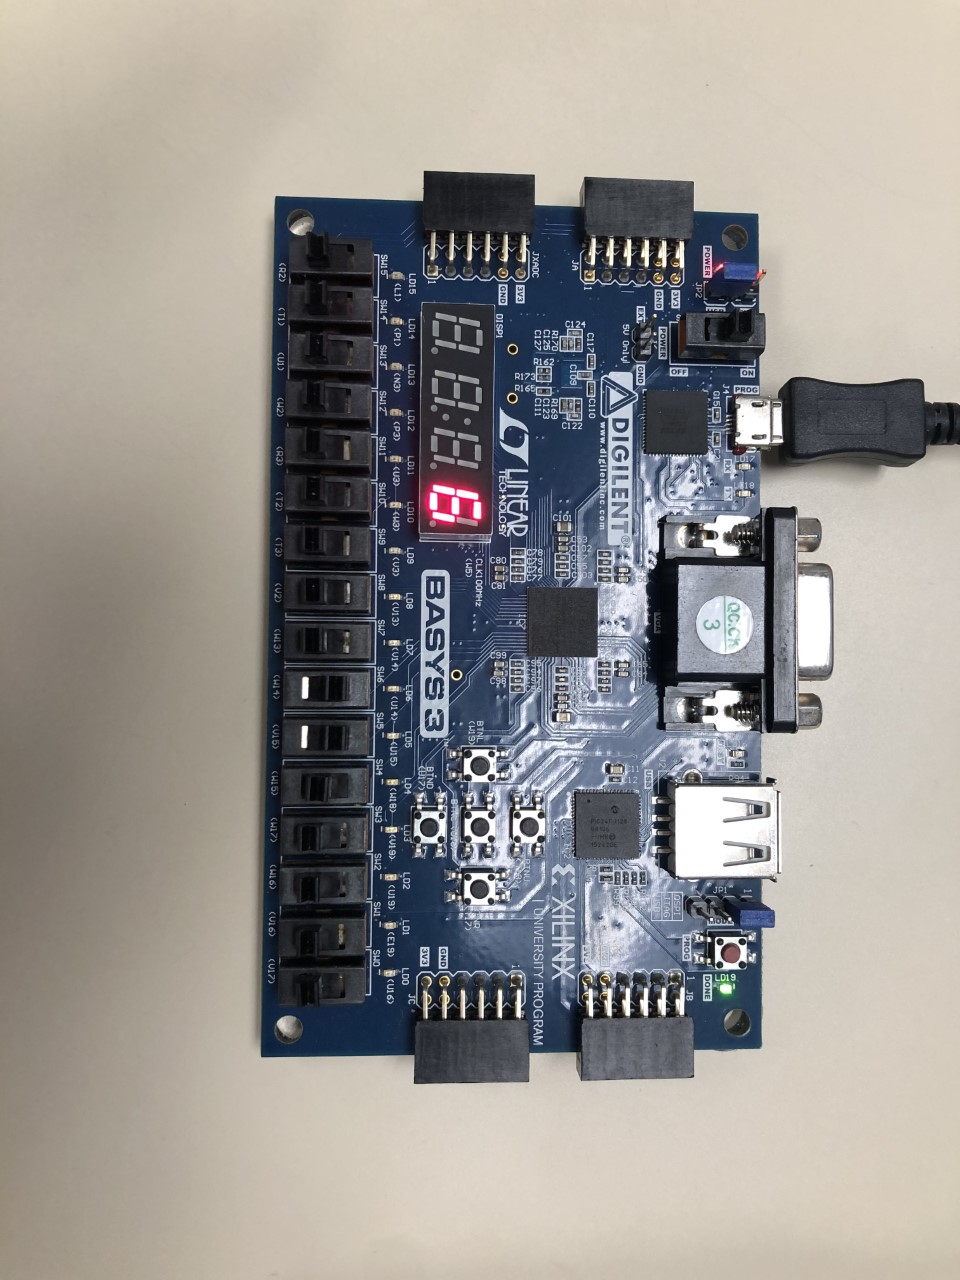
\includegraphics[width= \textwidth]{basys_.png}
	\caption{Basys board running 7 segment }\label{fig:Basys2}
\end{figure}

\end{document}
